\documentclass[HardwareDesign/HardwareDesign_main.tex]{subfiles}
\begin{document}
\section{Bolddispenser}
I det her afsnit vil der blive beskrevet de overvejelser, valg og udviklingsprocesser der skulle foretages under design af bolddispenser kredsløbet. Udvikling af komponenterne til bolddispenseren er baseret på prædefineret krav som kan læses under afsnittet Kravspecifikation (MANGLER REFERENCE!). Afsnittet er strukturet efter blockbeskrivelsen af bolddispenseren under afsnittet Arkitektur,Harwarearkitektur (MANGLER REFERENCE!).

\subsection{Bolddispenserens fysiske og mekaniske dele}
\subsubsection{Overvejelser}
Der findes mange mekaniske løsninger til dispensering af bolde. Den først metode som blev overvejet er den hvor to hjul sørger for at fremdrive bolden ud dispenseren, ligesom man gør med en tennis bolddispenser. Denne metode er dog mest brugt i tilfælde hvor der er behov for at få dispenseret bolden med en relativ høj hastighed. Fysisk fylder det også meget i forhold til nogle af de andre muligheder. Et andet løsning var at bruge den samme mekanisk system som bruges i typiske bordfodbolds borde. Fordelene er at man nemt kan finde en færdig design på nettet, og alle dele kan 3d printes. Ulempen er at der ikke bruges elektroniske aktuatorer.
Den tredje løsning som blev overvejet er en rotationsplatform mekanisme. Her udnytter man tyndekraften til at dispensere boldene. En cylinderformet beholder med et hul i bunden sider på den her roterende platform. For at dispensere boldene roteres platformen således at dens hul passer med hullet på bunden af cylinder-beholderen. Nå man så rotere igen, så bliver bolden i platformens hul dispenseret. Denne løsning er god fordi den bruger en aktuator til styring af dispensering, og den er simpel nok til at 3d printe. Ulempen er dog at platformen fylder meget.

\subsubsection{Valg}
Der valges platformløsningen da denne virker mest logisk. Fordi den mekaniske del er så simpel, så giver det rum til bedre udvikling af sensor og aktuator.

\subsubsection{Udviklingsproces}
Der købes ståltråde og gaffertape til udvikling af en pap prototype. Det er nødvendigt at lave en \textit{proof of concept} med en pap model før vi går i gang med alt andet. Der bruges tomme toiletpapirruller og køkkenruller til cylinder-beholderen. Under udvikling af beholderen blev jeg inspireret til at ændre mekanismen så der ikke var behov for en platform. I stedet for platformen skulle der være endnu en cylinderbeholder med et hul i siden. Denne mindre cylinder ville ligge under beholderen og holde boldene ind, ligesom platformen gjorde. For at dispensere bolde vil den rotere 180 grader rundt om beholderens højde-akse. Bolddispenseren bliver nu kompakt, mekanisk simpel, og nem at forbedre med aktuator og sensor. Boldispenserens fysisk konstruktion og dele kan ses på figur ????
(INDSÆT FIGUR!)
\subsection{Bolddispenserens Ball count sensor}
Denne sensor står for at notificere systemet om hvor vidt bolddispenseren har brug for flere bolde.
\subsubsection{Overvejelser}
Der var ikke mange overvejelser i forhold til denne sensor, da det var ret klart det skulle være en lyssensor. Boldene vejer for lidt til en pålidelig måling, og en kapacitans sensor er ikke praktisk i forhold til bolddispenserens fysiske dimensioner, fordi boldene ligger i et langt rør. Desuden er der meget mørk i bolddispenseren så en lyssensor vil ikke bliver forstyrret af så meget. I starten var det to lyssensorer der skulle placeres på bolddispenseren. En til at måle når bolddispenseren var ved at være tom og en anden til at måle når bolddispenseren var fyldt op. Men en endnu bedre løsning var kun at bruge en lyssensor der kunne måle afstande. På den måde kan man skrive et program der holder styr på afstanden og oversætter denne til et antal bolde.
\subsubsection{Valg}
Der valges at lave et lyssensor der kan måle afstand. For at undgå forstyringer under genopfyldningen af bolddispenseren, laves der et låg i toppen af bolddispenser beholderen hvor sensoren kan sidde.
\subsubsection{Udviklingsproces}
Der bruges en IR-emitter (SFH485) og en fotodiode (SFH203FA) til afstands sensoren. Det første vi gør er at undersøge hvordan fotodioden og IR-emitteren fungerer. Ind i datasheet for fotodioden står der en fotostrøm, som bliver genereret af fotodioden når den får infrarød lys. IR-emitterens opgave er at blinke ind bolddispenserens beholder så dens lys kan blive reflekteret af de bolde der er. Fotodioden skal vha. sin revers bias strøm oplyse os om hvor langt væk det først bold ramt af emitteren er, og dermed hvor mange bolde der er tilbage. Da fotodiodens revers bias strøm er afhængig af det effekt densitet som infrarødlys giver ($mW/cm^2$), så regner vi ikke med en lineær sammenhæng mellem afstand og fotostrøm.
Vi må ikke gå i gang med at teste uden først at tænke på, at forholdene ind i bolddispenseren er væsentlig anderledes end udenfor. Vi designer derfor et kredsløb som nemt kan re-dimensioneres efter behov. Vi vil gerne sikre os at vi kan måle forholdsvis store afstande. Derfor skal vi have den stærkeste lysintensitet vi kan få ud af IR-emitter. Vi kigger på datasheet og finder en graf for pulsevne, her aflæses at IR-emitteren kan tåle $1A$ i $100\mu s$ med en pulsbredde på $0.005$. Vi beregner vores pulsfrekvens til:
\[\frac{0.005}{100\mu s}=50Hz\]


\subsection{Bolddispenserens Coin collector}\label{subsec:bolddispenserensCoinCollector}
In this section the design choices and development of the hardware for the ball dispenser will be documented
\subsubsection{Overvejelser}
There are a lot of ways to implement a coin detection system, here some of the ideas we had will be presented.
The first option we considered was to have the coins go into a solid state sorting machine then fall on to a plate with a light sensor that would be covered by the coin which then triggers a mechanism to push the coins into the correct bins.
The second option considered was the coin falling down on some kind of pressure pad that works in the same manner as the option above.
The design we went with was the simplest one.
The coins fall down on two metal plates one connected to an interrupt on the PSOC with a pulldown to ground and the other at 5v.
So when the coin lands on the plate it bridges the connection and sends 5v to the interrupt, the coin is then collected or rejected by a stepper motor using a rotating disk with a hole in it (see figure \ref{})
\subsection{Design and development}\label{subsec:designAndDevelopment}
The sorting machine was designed in 3D using autodesk inventor pro.
It is built like a slide with precise holes in it to drop all coins but a 5kr though into the reject bin while the 5kr pass over and drop into the second hole where the coin is detected and possessed accordingly.
\begin{figure}
    \centering
    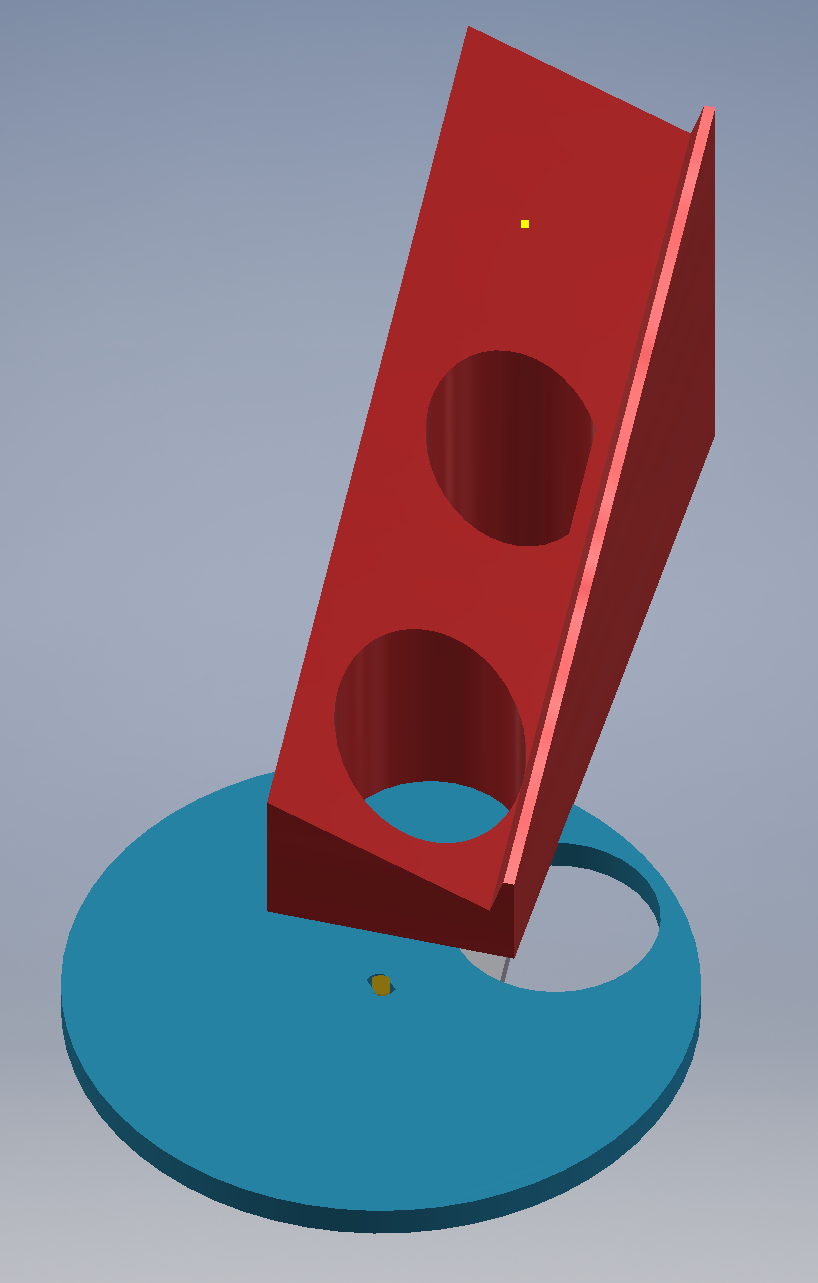
\includegraphics[width=\textwidth]{HardwareDesign/Bolddispenser/graphics/coinmaster.png}
    \caption{3D model of the coin collector (Top)}
    \label{fig:3D-CoinTop}
\end{figure}
\begin{figure}
    \centering
    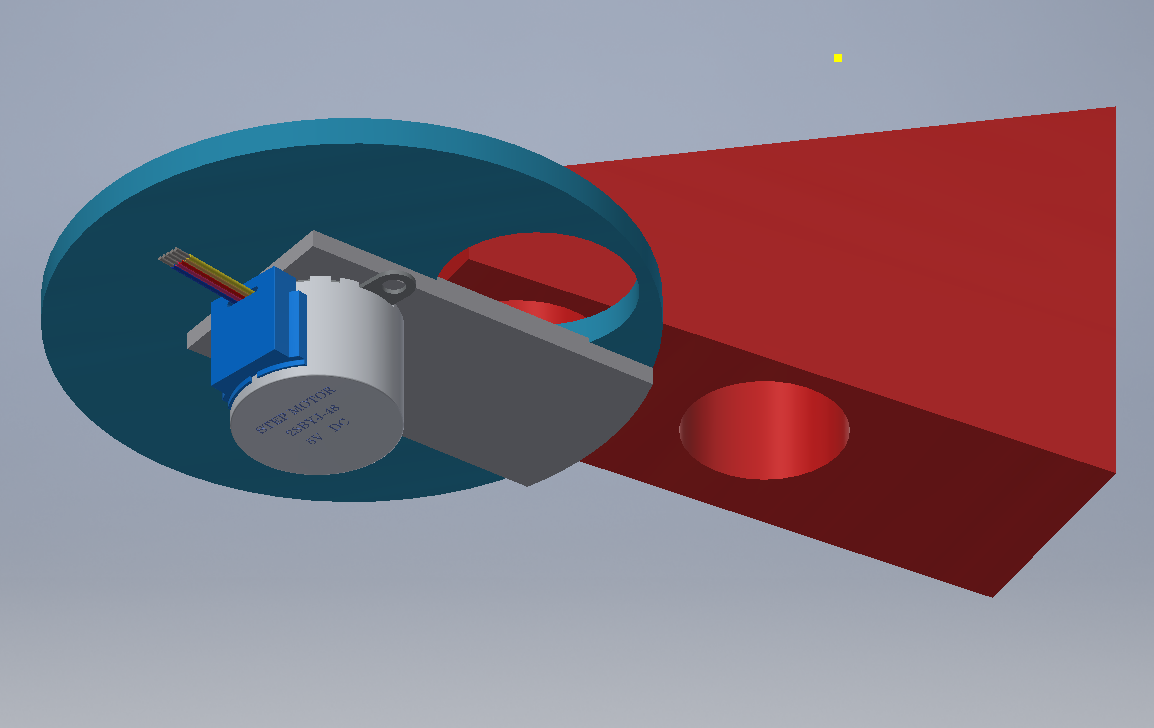
\includegraphics[width=\textwidth]{HardwareDesign/Bolddispenser/graphics/coinmaster-under.png}
    \caption{3D model of the coin collector (Bottom)}
    \label{fig:3D-CoinBottom}
\end{figure}
\end{document}